\section{Introduction}\label{sec:intro}
%======================================================================

Big Bang nucleosynthesis (BBN) is one of the three observational pillars of standard hot big bang cosmology, alongside the cosmic microwave background (CMB) and the Hubble expansion.  The standard calculation assumes a Friedmann--Lema\^itre--Robertson--Walker (FLRW) spacetime and has been developed to sub-percent precision by codes such as PRIMAT \cite{PitrouPRIMAT2021}, \textsc{PArthENoPE} \cite{PArthENoPE2018}, and \textsc{AlterBBN} \cite{AlterBBN2020}.  The predicted primordial helium-4 mass fraction $\Yp$ depends sensitively on the neutron lifetime $\tau_n$, the baryon-to-photon ratio $\eta$, the effective number of neutrino species $\Neff$, and the weak $n \leftrightarrow p$ interconversion rates.

Although the late-time universe is observationally very close to isotropic, that fact does not by itself exclude a significantly more anisotropic expansion history during the MeV era.  In BBN applications the relevant question is therefore not whether anisotropy exists today, but how much shear and anisotropic stress can be present at $T \sim 0.01$--$10\,\mathrm{MeV}$ without spoiling the primordial light-element yields.  The Bianchi classification provides the natural framework for spatially homogeneous but anisotropic cosmologies \cite{WainwrightEllis1997}.  For Type~I, the effect of anisotropy on BBN was first studied by Barrow \cite{Barrow1976}, while neutrino anisotropic stress (Misner viscosity) was incorporated by Rothman and Matzner \cite{RothmanMatzner1982}.  RABBIT currently provides implementation and diagnostic surfaces for this question; a precision BBN constraint remains an open B-01--B-06 objective.

RABBIT exposes a broader Type~I runtime core than the original SciPy-only framing of this report: (i) the SciPy Type~I reference as \texttt{backend="auto"} and number-of-record; (ii) an explicit bounded JAX tier-1 surface using live weak rates on the linearised Type~I transport surface; (iii) explicit exact-characteristic JAX surfaces (\texttt{"jax\_characteristic"} and \texttt{"jax\_characteristic\_tier2"}); and (iv) an explicit no-Teff JAX tier-3 weak-budget surface (\texttt{"jax\_advanced"}).  None is publication authority.  The report figures are historical diagnostics, and no finite-shear constraint is currently promoted.

\subsection{Runtime-scope declaration}

The strongest claims of this document apply to three distinct scope classes.
\begin{enumerate}
\item \textbf{Reference-result chain:} the exact-characteristic Type~I path that underlies the historical figures in this report, namely Type~I geometry, collisionless characteristic transport, live weak rates, Bennett QED thermodynamics, and the PRIMAT AC2024 network.
\item \textbf{Bounded registry-runtime surfaces:} the SciPy reference/fallback path, the JAX tier-1 live-weak surface, the explicit JAX exact-characteristic tier-1/tier-2 surfaces, and the no-Teff JAX tier-3 weak-budget surface, each with a declared metadata and runtime-regression contract but no publication-validation authority.
\item \textbf{Candidate or deferred perimeter:} Class~A / Class~B / tilted extensions, and full anisotropic collision-coupled Boltzmann/QKE closure.
\end{enumerate}

\subsection{Notation and scope guide}

\begin{table}[t]
\centering
\caption{Load-bearing notation used throughout the main production narrative.  The table is deliberately narrow: it lists the symbols that recur across geometry, transport, weak rates, and inference, and fixes their meanings at the report level.}\label{tab:notation}
\begin{tabularx}{0.95\textwidth}{@{}p{0.17\textwidth}X@{}}
\toprule
Symbol & Meaning \\
\midrule
$N=\ln a$ & e-fold time used as the independent variable of the production solve. \\
$\Sigma$ or $\Sigma_+$ & Hubble-normalised shear amplitude.  In the LRS Type~I production path one has $\Sigma_- = 0$. \\
$\Pi_\nu$ or $\Pi_+$ & Hubble-normalised neutrino anisotropic stress extracted from the characteristic rays. \\
$H/H_{\FLRW}$ & Hubble enhancement relative to the FLRW reference at the same plasma temperature. \\
$I_j, J_j, \Theta_j$ & Characteristic-ray energy shift, Jacobian, and per-ray effective temperature variables; explicit state variables on the SciPy reference path and analytic reconstructions on the compact JAX characteristic path. \\
$\tilde f_0(q)$ & Weak-rate-relevant monopole reconstructed from the characteristic rays. \\
$\lambda_{n\to p},\;\lambda_{p\to n}$ & Live weak interconversion rates evaluated from the current monopole and plasma state. \\
$\Neff$ & Effective neutrino-number diagnostic; in the production path this is helper-based rather than a fully anisotropic scattering-closed observable. \\
$\Delta\chi^2_{\rm prof}(\Sigma_H)$ & Profile statistic retained in the historical diagnostic grid; not a current validated constraint. \\
\bottomrule
\end{tabularx}
\end{table}

Figure~\ref{fig:story_chain} summarises the production logic used throughout the rest of the report.

\begin{figure*}[t]
\centering
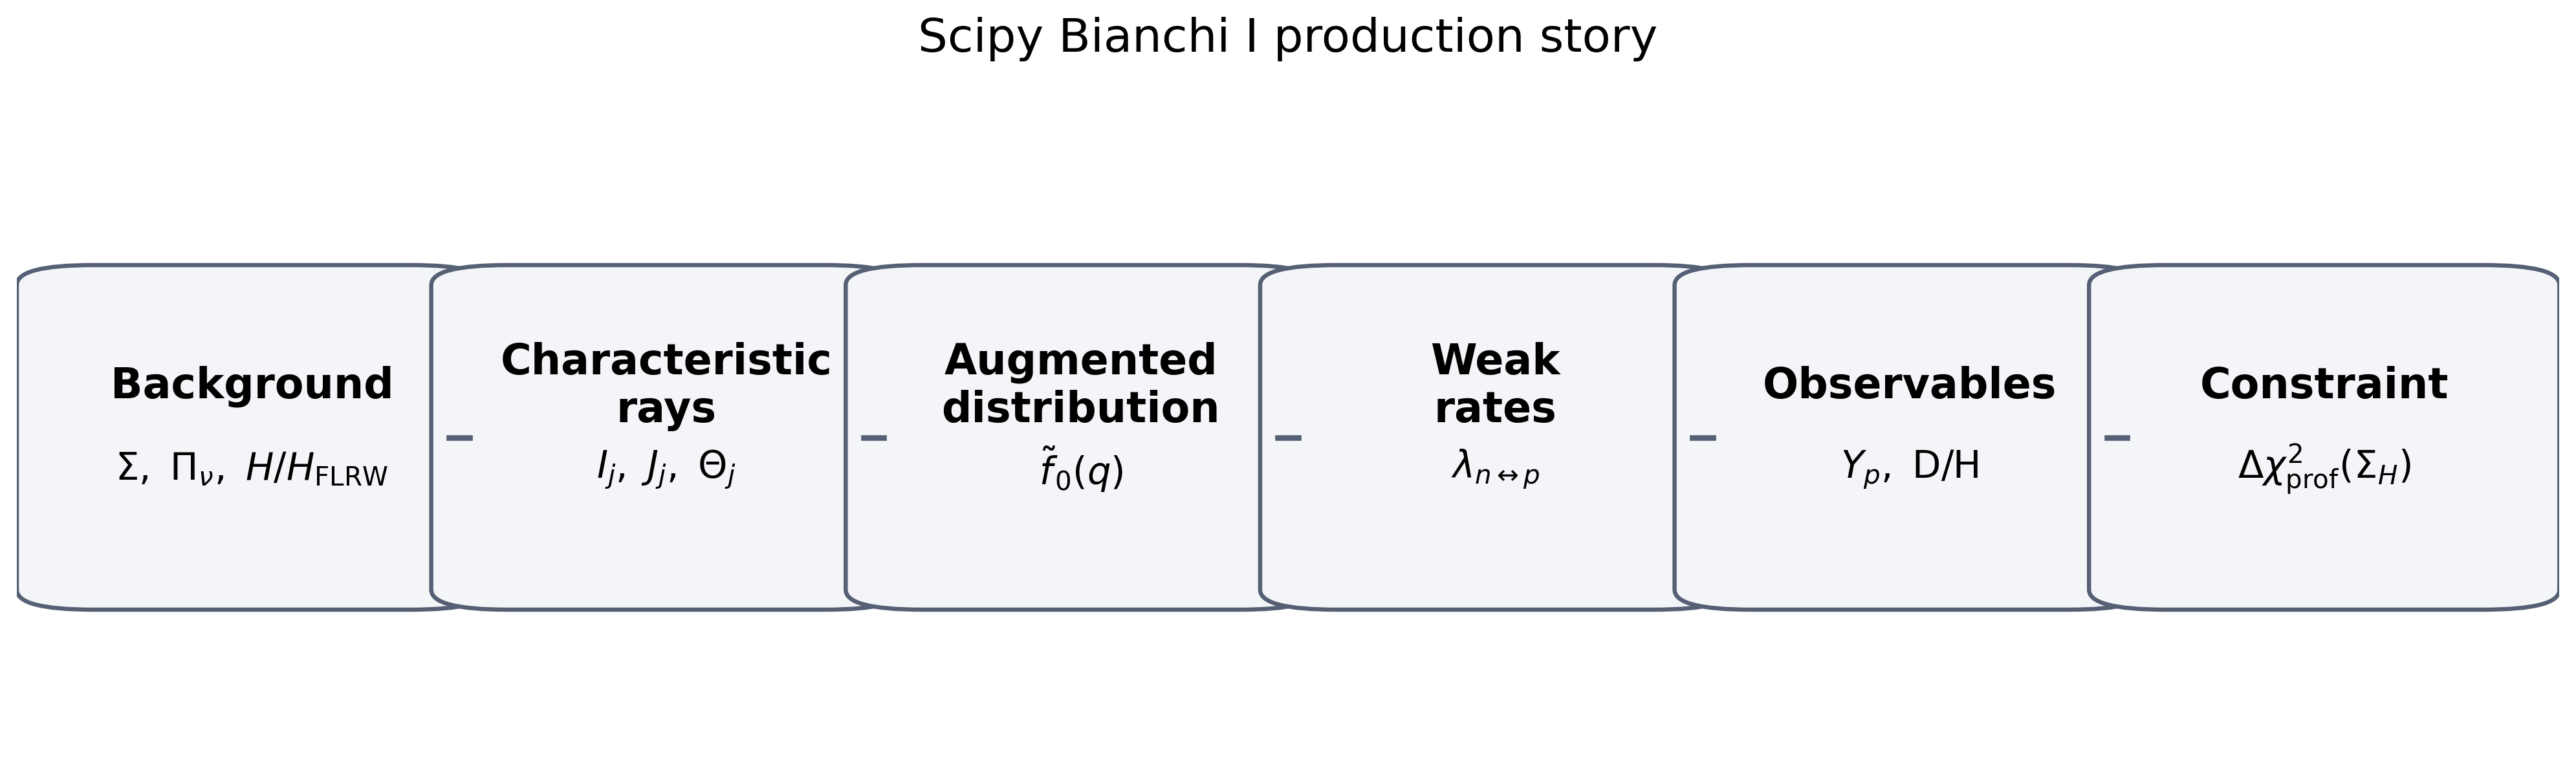
\includegraphics[width=\textwidth]{figures/fig_story_causal_chain.png}
\caption{Historical exact-characteristic diagnostic chain inside the current Type~I runtime core.  The chain runs from geometry through characteristic transport and the augmented monopole to weak rates, BBN observables, and a legacy profile readout.  It is a roadmap for future falsification, not evidence for a current finite-shear constraint.}
\label{fig:story_chain}
\end{figure*}

\subsection{Outline}

Part~I (Foundations) covers the Bianchi geometry (\S\ref{sec:geometry}), collisionless neutrino transport (\S\ref{sec:transport}), the eigenvalue structure (\S\ref{sec:eigenvalues}), a brief historical note on the effective-temperature framework (\S\ref{sec:teff}), and the exact characteristic method (\S\ref{sec:characteristic}).

Part~II (Collision Physics) presents the collision-side scaffolding that is relevant for understanding the tiered incomplete-decoupling story: the collision-integral structure (\S\ref{sec:collision_integral}), the Hannestad--Madsen kernel (\S\ref{sec:hannestad_madsen}), the relaxation-time approximation (\S\ref{sec:rta}), and the incomplete-decoupling hierarchy (\S\ref{sec:incomplete_decoupling}).

Part~III (Production Pipeline) covers weak rates (\S\ref{sec:weak}), the QED equation of state (\S\ref{sec:qed}), the nuclear network (\S\ref{sec:network}), the solver architecture (\S\ref{sec:solver}), the coupled production system (\S\ref{sec:coupled}), results (\S\ref{sec:results}), validation (\S\ref{sec:validation}), discussion (\S\ref{sec:discussion}), and the appendices that supply reference derivations and developer-facing implementation maps.

%======================================================================
